%%%%%%%%%%%%%%%%%%%%%%%%%%%%%%%%%%%%%%%%%%%%%%%%%%%%%%%%%%%%%%%%%%%%%%%%%%%

\documentclass{standalone}

\usepackage{amsmath}
\usepackage{mathptmx}
\usepackage{pgfplots}
\usetikzlibrary{external}
\tikzexternalize{damped}
\pgfplotsset{compat=1.16}

%% IEEE uses Times Roman font, so we'll default to Times.
%% These three commands make up the entire times.sty package.
\renewcommand{\rmdefault}{ptm}
\renewcommand{\ttdefault}{pcr}
\normalfont\selectfont

\begin{document}

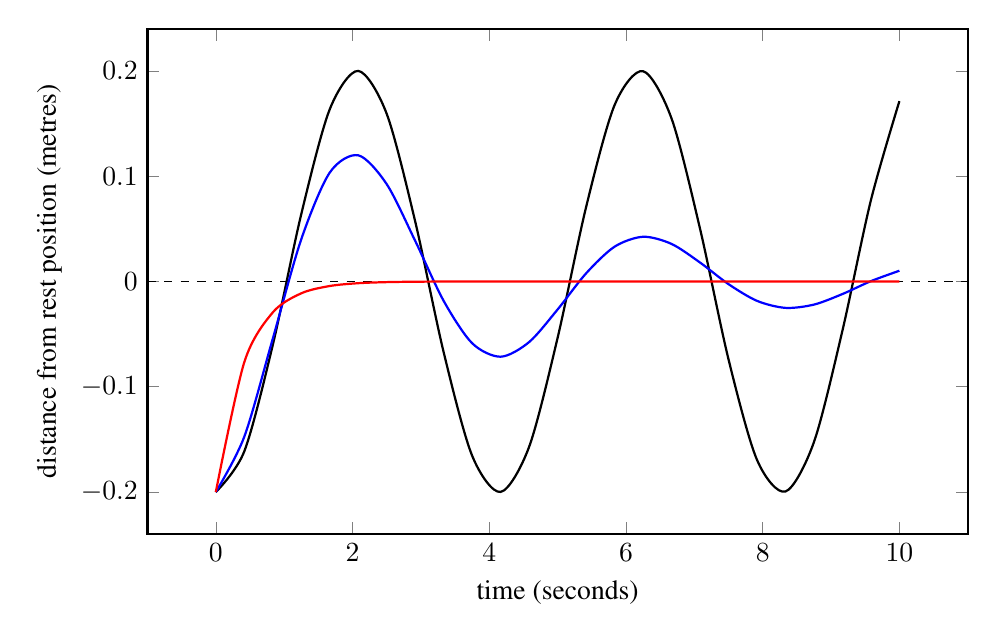
\begin{tikzpicture}
\tikzset{%%
  every mark/.append style={scale=1.0},%%
  scale=1.0%%
}
\pgfplotsset{%%
  every axis/.append style={font=\normalsize}%%
}

\begin{axis}[%%
  axis line style=thick,%%
  enlargelimits=true,%%
  height=8cm,%%
  plotStyle/.style={%%
    domain=0:10,%%
    mark=none,%%
    smooth,%%
    thick%%
  },%%
  width=12cm,%%
  %%
  %% x-axis
  xlabel={\normalsize time~(seconds)},%%
  %%
  %% y-axis
  ylabel={\normalsize distance from rest position~(metres)},%%
  ylabel style=above%%
]
%%
%%
%% Horizontal line through the origin.
\draw[thin,dashed] (axis cs:\pgfkeysvalueof{/pgfplots/xmin},0) -- (axis cs:\pgfkeysvalueof{/pgfplots/xmax},0);
%%
%%
%% Displacement when b = 0, no friction.
\addplot+ [plotStyle,black]
{-0.2 * cos(deg(sqrt(2.3) * x))};
%%
%%
%% Displacement when b = km, underdamped.
\addplot+ [plotStyle,blue]
{-0.2 * exp(-0.245 * x) * cos(deg(sqrt(2.3 - 0.345^2) * x))};
%%
%%
%% Displacement when b = 2m sqrt(k/m), critically damped.
\addplot+ [plotStyle,red]
{-0.2 * exp(-2.3 * x)};
\end{axis}
\end{tikzpicture}

\end{document}
